%*============================================================*
%**Goal		:    文献分享:消失的女性与茶叶的价格
%**Author	:  	 ZhangYi zhangyiceee@163.com 15592606739
%**Created	:  	 20200323
%**Last Modified: 2020
%*============================================================*



\documentclass{beamer}
\usepackage[UTF8,noindent]{ctexcap}
\usepackage{natbib}
\usepackage{hyperref}


\graphicspath{{figures/}}




\usetheme{Madrid}
%\usecolortheme{crane} %黄色
%\usecolortheme{wolverine} %黄蓝
\usecolortheme{lily} %蓝白
%\usecolortheme{beetle} %灰色
%Information to be included in the title page:
\title[文献分享:ZY]{Early Life Circumstance and Adult Mental Health}
\author[Achyuta et al.]{Achyuta Adhvaryu;James Fenske;Anant Nyshadham}
\date{\today}

\begin{document}

\frame{\titlepage}
%开始你的表演



%第1页幻灯片
%==========================================
\begin{frame}
\frametitle{Abstract}
We show that psychological well-being in adulthood varies with circumstance in early life. Combining a time series of real producer prices of cocoa with a nationally representative household survey in Ghana, we find that a one standard deviation rise in the cocoa price in early life decreases the likelihood of severe mental distress in adulthood by 3 percentage points (half the mean prevalence) for cohorts born in cocoa-producing regions relative to those born in other regions. Impacts on related personality traits are consistent with this result. Maternal nutrition, reinforcing childhood investments, and adult circumstance are likely operative channels of impact.
\citep{Almond2019}\citet{Adhvaryu2019}
\end{frame}



\begin{frame}
    \frametitle{Problem}
心理健康问题占全球疾病的13\%,这些疾病主要发生在低收入地区,因此研究心理健康的根源所在显得尤为重要,大多数文献研究的是收入和客观健康之间的复杂关系,比较少的一部分文献研究的是同期的家庭居住条件变化在当期的影响,很少有文献研究其长期影响。
\end{frame}

\begin{frame}
    \frametitle{Objective}
How does circumstance in early life affect psychological distress in adulthood?
\\ 早期环境变化如何影响成年后的心理健康?
\\ We exploit variation in early life conditions induced by changes in the real producer price of cocoa. Cocoa is Ghana’s chief agricultural export commodity, and its price is a key determinant of household incomes in the regions where it is grown.
\end{frame}



\begin{frame}
    \frametitle{Result}
    在加纳那些种植可可的地区,个体出生时低的可可价格提高了个体成年后患严重精神压力发生率。
    \\ 可可价格降低一个标准差,种植可可地区出生的孩子与没有种植可可地区出生的孩子相比患有严重精神压力的可能性提高了3个百分点。
\end{frame}


\begin{frame}
    \frametitle{机制分析}
    \begin{itemize}
    	\item 通过数据发现,可可价格能积极预测母亲的健康和BMI,而母亲的健康和BMI与孩子出生时的健康高度相关;
    	\item 父母通过提高疫苗接种率和延长母乳喂养时间来强化孩子初始禀赋
    	\item 以身高衡量的健康状况随可可价格的提高而明显改善,但经济状况指标(储蓄和职业类型)并没有明显提高。
    \end{itemize}
\end{frame}


\begin{frame}
    \frametitle{Additional}
    还发现死亡率和生育率都会对价格作出反应,因此要研究选择死亡了生育在多大程度上影响心理健康方面估计结果
    \begin{itemize}
    	\item 在控制父母的特征(受教育程度、职业的虚拟变量)后影响大小没变化;
    	\item 加入家庭固定效应,效果更大了
    	\item 没看懂
    \end{itemize}
\end{frame}

\begin{frame}
	\frametitle{以往研究}
	经济学领域内的文献很少,在医学领域有研究对长期心理健康的影响,但是X都是极端恶劣环境的影响(饥荒),经济学研究中最接近的时由于近亲死亡造成的母亲精神紧张的影响,发现:孩子在童年和成年时期因精神健康障碍而使用处方药的情况大幅增加;
	\\ 文中列出得饥荒文献:Brown et al. (1995, 2000); Hoek et al. (1998, 1996); Huang et al. (2013); Neugebauer et al. (1999); Pol et al. (2000); Susser and Lin (1992). This evidence focuses overwhelmingly on the impacts of severe famines, particularly on the case of the Dutch Winter Famine of 1944-1945.

\end{frame}

\begin{frame}
	\frametitle{以往研究}
	本文关注的心理健康和文献中的人格特征以及非认知能力比较接近。
\end{frame}

\begin{frame}
	\frametitle{Empirical strategy}
	\begin{itemize}
		\item 直觉
		\item 动机
		\item Specification
	\end{itemize}
\end{frame}

\begin{frame}
	\frametitle{直觉}
	The intuition for our identification strategy is that households in the cocoa-producing regions of Ghana experience changes in the real producer price of cocoa as income shocks,while households in regions that do not produce cocoa are unaffected by these fluctuations. Children born into households in cocoa-growing regions during periods of high cocoa prices will have more resources, owing both to the higher incomes of cocoa-producing households and to the dependence of non-agricultural activities in these regions on the cocoa sector. These resource booms could have large and lasting impacts on mental health through their effects during both gestation and infancy.
\end{frame}

\begin{frame}
	\frametitle{动机}
	\centering
	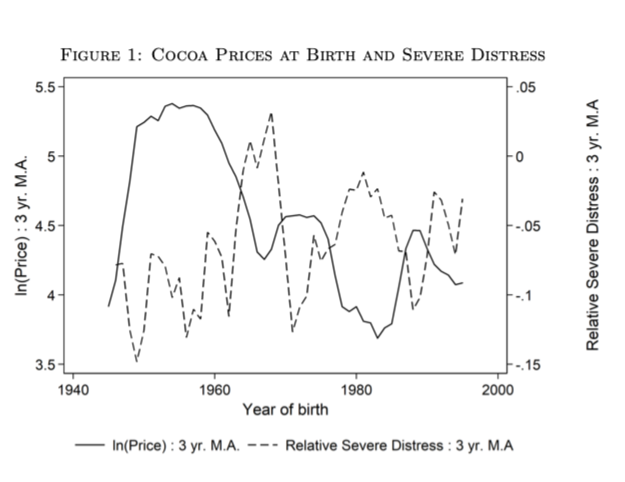
\includegraphics[scale=0.5]{figure1}
\end{frame}

\begin{frame}
	\frametitle{动机}
	That is, individuals born in the cocoaproducing regions of Ghana when incomes of cocoa-producers are high show low rates of severe mental distress relative to individuals born in the same year but in parts of Ghana that do not grow cocoa. When incomes in cocoa-producing regions fall, the pattern is reversed.
\end{frame}

\begin{frame}
	\frametitle{Specification}
	$$Outcome_{irt} = \alpha + \beta (CocoaPrice_t)CocoaProducer_r +x'_{irt}\gamma+\delta_r+\eta_t+\epsilon_{irt}$$
$x'_{irt}$代表一系列控制变量,性别、是否为户主、性别和户主交互项目、地区的虚拟变量,$\delta_r \eta_t$分别代表年份和地区的固定效应,$(CocoaPrice_t)CocoaProducer_r$成为价格冲击。


\end{frame}
\begin{frame}
	\frametitle{3:Data}
	\begin{itemize}
		\item Cocoa prices and production:没看懂
		\item Mental health :主要介绍心理健康的量表
		\item Additional controls :介绍一系列控制变量,值的注意的是作者增加了降雨和温度变化的控制变量
		\item Demographic and health survey data
		\begin{itemize}
			\item 女性的出生年份、居住地、受教育程度、农村、年龄、职业、地区、种族、身高体重
			\item 女性生育史的完整数据,孩子的出生年、出生顺序、性别、是否还活着、如果死亡,那么活了多久
			\item 孩子的重新编码:包括孩子的出生年份、出生顺序、多胎、性别和孩子目前的月龄等信息。最重要的是,母亲们会被问及早期生活的投资情况,如这些孩子的疫苗接种史以及他们接受母乳喂养的时间。母亲们还被问及产前投资,如看医生、额外的疫苗接种以及分娩情况。
		\end{itemize}
		\item 人口普查数据
		\item 描述性统计
	\end{itemize}
\end{frame}

\begin{frame}
	\frametitle{描述性统计结果}
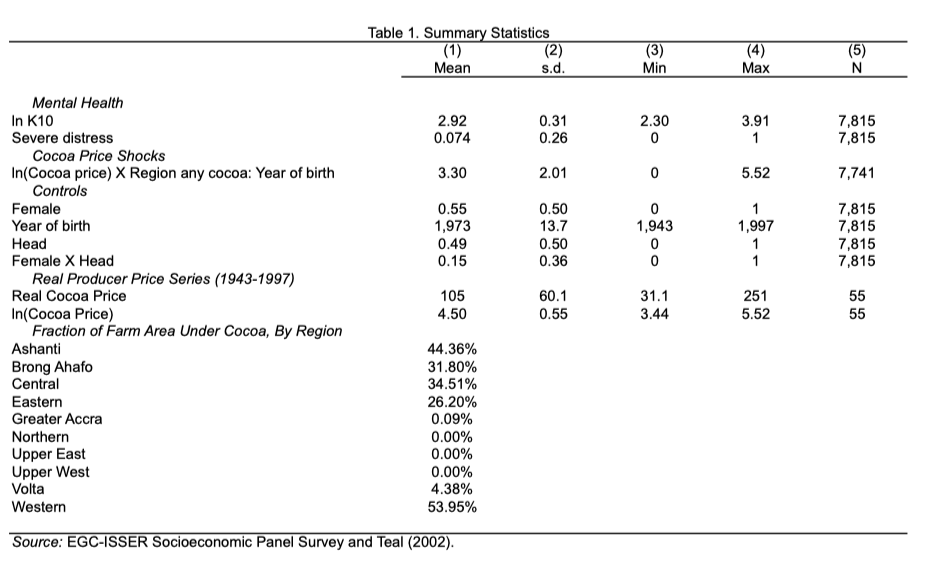
\includegraphics[scale=0.35]{figures/table1.png}	
\end{frame}
\begin{frame}
	\frametitle{Result}
	\begin{itemize}
		\item 4.1 Mental Distress
		\item 4.2 Personality Outcomes
		\item 4.3 机制-{不讲}
	\end{itemize}

\end{frame}

\begin{frame}
	\frametitle{4.1 Mental Distress}
	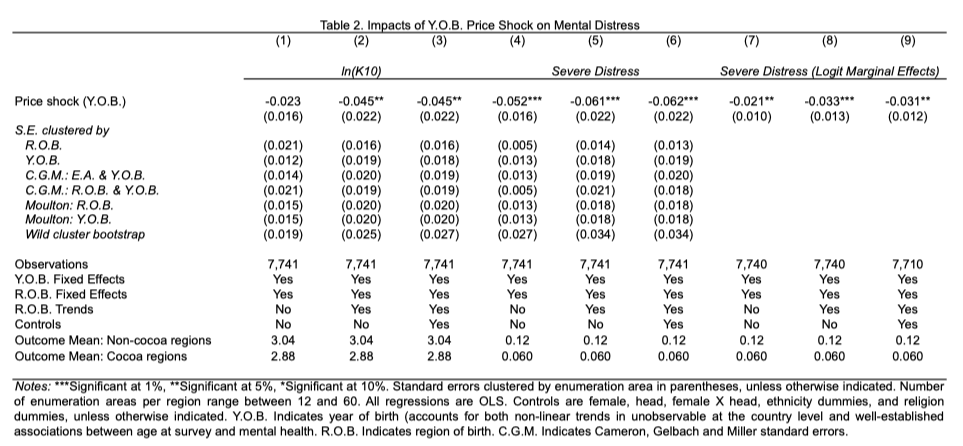
\includegraphics[scale=0.35]{figures/table2.png}
\end{frame}

\begin{frame}
	\frametitle{4.2 Personality Outcomes}
	\centering{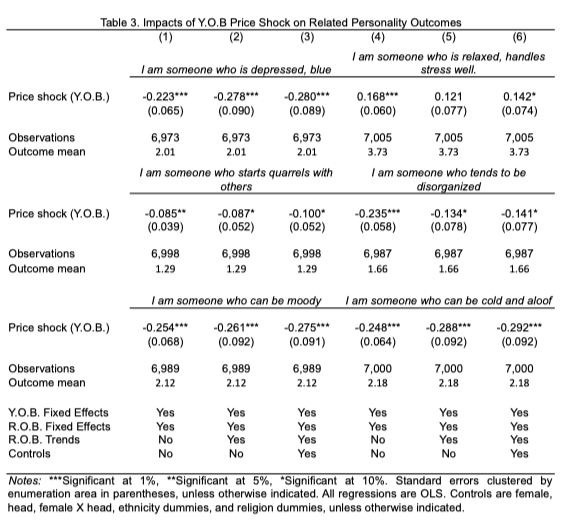
\includegraphics[scale=0.4]{figures/table3.png}}
\end{frame}


\begin{frame}
	\frametitle{5 Conclusion}
负面影响
\end{frame}




\begin{frame}
    \frametitle{参考文献}
\bibliographystyle{plainnat}
\bibliography{references}
\end{frame}

%参考文献的案例 \citet{Krueger1999Experimental} \citep{Krueger1999Experimental}  注意两类的不同
\end{document}



